\documentclass[]{article}
\usepackage{lmodern}
\usepackage{amssymb,amsmath}
\usepackage{ifxetex,ifluatex}
\usepackage{fixltx2e} % provides \textsubscript
\ifnum 0\ifxetex 1\fi\ifluatex 1\fi=0 % if pdftex
  \usepackage[T1]{fontenc}
  \usepackage[utf8]{inputenc}
\else % if luatex or xelatex
  \ifxetex
    \usepackage{mathspec}
  \else
    \usepackage{fontspec}
  \fi
  \defaultfontfeatures{Ligatures=TeX,Scale=MatchLowercase}
\fi
% use upquote if available, for straight quotes in verbatim environments
\IfFileExists{upquote.sty}{\usepackage{upquote}}{}
% use microtype if available
\IfFileExists{microtype.sty}{%
\usepackage{microtype}
\UseMicrotypeSet[protrusion]{basicmath} % disable protrusion for tt fonts
}{}
\usepackage[margin=1in]{geometry}
\usepackage{hyperref}
\hypersetup{unicode=true,
            pdftitle={Processing, cleaning and saving NZ GREEN Grid project time use diary data},
            pdfauthor={Ben Anderson (b.anderson@soton.ac.uk, @dataknut)},
            pdfborder={0 0 0},
            breaklinks=true}
\urlstyle{same}  % don't use monospace font for urls
\usepackage{color}
\usepackage{fancyvrb}
\newcommand{\VerbBar}{|}
\newcommand{\VERB}{\Verb[commandchars=\\\{\}]}
\DefineVerbatimEnvironment{Highlighting}{Verbatim}{commandchars=\\\{\}}
% Add ',fontsize=\small' for more characters per line
\usepackage{framed}
\definecolor{shadecolor}{RGB}{248,248,248}
\newenvironment{Shaded}{\begin{snugshade}}{\end{snugshade}}
\newcommand{\KeywordTok}[1]{\textcolor[rgb]{0.13,0.29,0.53}{\textbf{#1}}}
\newcommand{\DataTypeTok}[1]{\textcolor[rgb]{0.13,0.29,0.53}{#1}}
\newcommand{\DecValTok}[1]{\textcolor[rgb]{0.00,0.00,0.81}{#1}}
\newcommand{\BaseNTok}[1]{\textcolor[rgb]{0.00,0.00,0.81}{#1}}
\newcommand{\FloatTok}[1]{\textcolor[rgb]{0.00,0.00,0.81}{#1}}
\newcommand{\ConstantTok}[1]{\textcolor[rgb]{0.00,0.00,0.00}{#1}}
\newcommand{\CharTok}[1]{\textcolor[rgb]{0.31,0.60,0.02}{#1}}
\newcommand{\SpecialCharTok}[1]{\textcolor[rgb]{0.00,0.00,0.00}{#1}}
\newcommand{\StringTok}[1]{\textcolor[rgb]{0.31,0.60,0.02}{#1}}
\newcommand{\VerbatimStringTok}[1]{\textcolor[rgb]{0.31,0.60,0.02}{#1}}
\newcommand{\SpecialStringTok}[1]{\textcolor[rgb]{0.31,0.60,0.02}{#1}}
\newcommand{\ImportTok}[1]{#1}
\newcommand{\CommentTok}[1]{\textcolor[rgb]{0.56,0.35,0.01}{\textit{#1}}}
\newcommand{\DocumentationTok}[1]{\textcolor[rgb]{0.56,0.35,0.01}{\textbf{\textit{#1}}}}
\newcommand{\AnnotationTok}[1]{\textcolor[rgb]{0.56,0.35,0.01}{\textbf{\textit{#1}}}}
\newcommand{\CommentVarTok}[1]{\textcolor[rgb]{0.56,0.35,0.01}{\textbf{\textit{#1}}}}
\newcommand{\OtherTok}[1]{\textcolor[rgb]{0.56,0.35,0.01}{#1}}
\newcommand{\FunctionTok}[1]{\textcolor[rgb]{0.00,0.00,0.00}{#1}}
\newcommand{\VariableTok}[1]{\textcolor[rgb]{0.00,0.00,0.00}{#1}}
\newcommand{\ControlFlowTok}[1]{\textcolor[rgb]{0.13,0.29,0.53}{\textbf{#1}}}
\newcommand{\OperatorTok}[1]{\textcolor[rgb]{0.81,0.36,0.00}{\textbf{#1}}}
\newcommand{\BuiltInTok}[1]{#1}
\newcommand{\ExtensionTok}[1]{#1}
\newcommand{\PreprocessorTok}[1]{\textcolor[rgb]{0.56,0.35,0.01}{\textit{#1}}}
\newcommand{\AttributeTok}[1]{\textcolor[rgb]{0.77,0.63,0.00}{#1}}
\newcommand{\RegionMarkerTok}[1]{#1}
\newcommand{\InformationTok}[1]{\textcolor[rgb]{0.56,0.35,0.01}{\textbf{\textit{#1}}}}
\newcommand{\WarningTok}[1]{\textcolor[rgb]{0.56,0.35,0.01}{\textbf{\textit{#1}}}}
\newcommand{\AlertTok}[1]{\textcolor[rgb]{0.94,0.16,0.16}{#1}}
\newcommand{\ErrorTok}[1]{\textcolor[rgb]{0.64,0.00,0.00}{\textbf{#1}}}
\newcommand{\NormalTok}[1]{#1}
\usepackage{longtable,booktabs}
\usepackage{graphicx,grffile}
\makeatletter
\def\maxwidth{\ifdim\Gin@nat@width>\linewidth\linewidth\else\Gin@nat@width\fi}
\def\maxheight{\ifdim\Gin@nat@height>\textheight\textheight\else\Gin@nat@height\fi}
\makeatother
% Scale images if necessary, so that they will not overflow the page
% margins by default, and it is still possible to overwrite the defaults
% using explicit options in \includegraphics[width, height, ...]{}
\setkeys{Gin}{width=\maxwidth,height=\maxheight,keepaspectratio}
\IfFileExists{parskip.sty}{%
\usepackage{parskip}
}{% else
\setlength{\parindent}{0pt}
\setlength{\parskip}{6pt plus 2pt minus 1pt}
}
\setlength{\emergencystretch}{3em}  % prevent overfull lines
\providecommand{\tightlist}{%
  \setlength{\itemsep}{0pt}\setlength{\parskip}{0pt}}
\setcounter{secnumdepth}{5}
% Redefines (sub)paragraphs to behave more like sections
\ifx\paragraph\undefined\else
\let\oldparagraph\paragraph
\renewcommand{\paragraph}[1]{\oldparagraph{#1}\mbox{}}
\fi
\ifx\subparagraph\undefined\else
\let\oldsubparagraph\subparagraph
\renewcommand{\subparagraph}[1]{\oldsubparagraph{#1}\mbox{}}
\fi

%%% Use protect on footnotes to avoid problems with footnotes in titles
\let\rmarkdownfootnote\footnote%
\def\footnote{\protect\rmarkdownfootnote}

%%% Change title format to be more compact
\usepackage{titling}

% Create subtitle command for use in maketitle
\newcommand{\subtitle}[1]{
  \posttitle{
    \begin{center}\large#1\end{center}
    }
}

\setlength{\droptitle}{-2em}
  \title{Processing, cleaning and saving NZ GREEN Grid project time use diary
data}
  \pretitle{\vspace{\droptitle}\centering\huge}
  \posttitle{\par}
  \author{Ben Anderson
(\href{mailto:b.anderson@soton.ac.uk}{\nolinkurl{b.anderson@soton.ac.uk}},
\texttt{@dataknut})}
  \preauthor{\centering\large\emph}
  \postauthor{\par}
  \predate{\centering\large\emph}
  \postdate{\par}
  \date{Last run at: 2018-05-10 17:40:56}


\begin{document}
\maketitle

{
\setcounter{tocdepth}{2}
\tableofcontents
}
\newpage

\section{Citation}\label{citation}

If you wish to use any of the material from this report please cite as:

\begin{itemize}
\tightlist
\item
  Anderson, B. (2018) Processing, cleaning and saving NZ GREEN Grid
  project time use diary data, University of Otago: Dunedin, NZ.
\end{itemize}

\newpage

\section{Introduction}\label{introduction}

Report circulation:

\begin{itemize}
\tightlist
\item
  Restricted to:
  \href{https://www.otago.ac.nz/centre-sustainability/research/energy/otago050285.html}{NZ
  GREEn Grid} project partners and contractors.
\end{itemize}

\subsection{Purpose}\label{purpose}

This report is intended to:

\begin{itemize}
\tightlist
\item
  load and clean the two time use survey datasets
\item
  save the cleaned data out to /Volumes/hum-csafe/Research
  Projects/GREEN Grid/Clean\_data/safe/TUD/ as two seperate files, one
  for each survey
\item
  produce summary data quality statistics
\end{itemize}

\subsection{Requirements:}\label{requirements}

Time use survey data held in /Volumes/hum-csafe/Research Projects/GREEN
Grid/\_RAW DATA/Time Use Diaries/:

\begin{itemize}
\tightlist
\item
  PowerCo
\item
  Unison
\end{itemize}

A lookup table to correct mis-coding of household IDs
(/Volumes/hum-csafe/Research Projects/GREEN Grid/\_RAW
DATA/TUD\_2\_GridSpyLookup.xlsx).

\subsection{History}\label{history}

Generally tracked via our git.soton
\href{https://git.soton.ac.uk/ba1e12/nzGREENGrid}{repo}:

\begin{itemize}
\tightlist
\item
  \href{https://git.soton.ac.uk/ba1e12/nzGREENGrid/commits/master}{history}
\item
  \href{https://git.soton.ac.uk/ba1e12/nzGREENGrid/issues}{issues}
\end{itemize}

\subsection{Support}\label{support}

This work was supported by:

\begin{itemize}
\tightlist
\item
  The \href{https://www.otago.ac.nz/}{University of Otago}
\item
  The New Zealand \href{http://www.mbie.govt.nz/}{Ministry of Business,
  Innovation and Employment (MBIE)}
\item
  \href{http://www.energy.soton.ac.uk/tag/spatialec/}{SPATIALEC} - a
  \href{http://ec.europa.eu/research/mariecurieactions/about-msca/actions/if/index_en.htm}{Marie
  Skłodowska-Curie Global Fellowship} based at the University of Otago's
  \href{http://www.otago.ac.nz/centre-sustainability/staff/otago673896.html}{Centre
  for Sustainability} (2017-2019) \& the University of Southampton's
  Sustainable Energy Research Group (2019-202).
\end{itemize}

This work is (c) 2018 the University of Southampton.

We do not `support' the code but if you have a problem check the
\href{https://git.soton.ac.uk/ba1e12/nzGREENGrid/issues}{issues} on our
\href{https://git.soton.ac.uk/ba1e12/nzGREENGrid}{repo} and if it
doesn't already exist, open one. We might be able to fix it :-)

\section{Load files}\label{load-files}

In this section we load and test the two time-use survey datasets.

\subsection{PowerCo}\label{powerco}

This consists of 1 file found in /Volumes/hum-csafe/Research
Projects/GREEN Grid/\_RAW DATA/Time Use Diaries/Powerco/Powerco
Annexes/:

\begin{itemize}
\tightlist
\item
  TUD (Merged data)\_BA.csv
\end{itemize}

This is a version of TUD (Merged data).csv with:

\begin{itemize}
\tightlist
\item
  small edits to correct dates
\item
  redundant rows removed from file header
\end{itemize}

\begin{Shaded}
\begin{Highlighting}[]
\NormalTok{tudPowerCoDT <-}\StringTok{ }\KeywordTok{fread}\NormalTok{(}\KeywordTok{paste0}\NormalTok{(powerCoPath, }\StringTok{"TUD (Merged data)_BA.csv"}\NormalTok{))}

\NormalTok{nRows <-}\StringTok{ }\KeywordTok{nrow}\NormalTok{(tudPowerCoDT)}
\KeywordTok{print}\NormalTok{(}\KeywordTok{paste0}\NormalTok{(}\StringTok{"Found "}\NormalTok{, }\KeywordTok{tidyNum}\NormalTok{(nRows), }\StringTok{" rows of data"}\NormalTok{))}
\end{Highlighting}
\end{Shaded}

\begin{verbatim}
## [1] "Found 352 rows of data"
\end{verbatim}

\begin{Shaded}
\begin{Highlighting}[]
\CommentTok{# Remove identifying data ----}
\NormalTok{tudPowerCoDT <-}\StringTok{ }\NormalTok{tudPowerCoDT[, }\KeywordTok{c}\NormalTok{(}\StringTok{"RowNum"}\NormalTok{, }\StringTok{"Name"}\NormalTok{,}\StringTok{"EmailAddress"}\NormalTok{) }\OperatorTok{:}\ErrorTok{=}\StringTok{ }\OtherTok{NULL}\NormalTok{]}

\CommentTok{# Fix names of variables ----}
\NormalTok{tudPowerCoDT <-}\StringTok{ }\NormalTok{data.table}\OperatorTok{::}\KeywordTok{setnames}\NormalTok{(tudPowerCoDT, }
                                    \KeywordTok{c}\NormalTok{(}\StringTok{"Family size"}\NormalTok{, }\StringTok{"Choose the date of your diary / entry:"}\NormalTok{), }
                                    \KeywordTok{c}\NormalTok{(}\StringTok{"ba_nPeople"}\NormalTok{, }\StringTok{"diaryDate"}\NormalTok{)}
\NormalTok{)}

\CommentTok{# Fix dates ----}
\NormalTok{tudPowerCoDT <-}\StringTok{ }\NormalTok{tudPowerCoDT[, r_diaryDate }\OperatorTok{:}\ErrorTok{=}\StringTok{ }\NormalTok{lubridate}\OperatorTok{::}\KeywordTok{mdy}\NormalTok{(diaryDate)]}

\CommentTok{# Fix the hhid}
\NormalTok{tudPowerCoDT <-}\StringTok{ }\NormalTok{tudPowerCoDT[, hhID }\OperatorTok{:}\ErrorTok{=}\StringTok{ }\KeywordTok{paste0}\NormalTok{(}\StringTok{"rf_"}\NormalTok{, HHCODE)]}
\NormalTok{tudPowerCoDT <-}\StringTok{ }\NormalTok{tudPowerCoDT[, hhID }\OperatorTok{:}\ErrorTok{=}\StringTok{ }\KeywordTok{ifelse}\NormalTok{(}\KeywordTok{as.integer}\NormalTok{(HHCODE) }\OperatorTok{<}\StringTok{ }\DecValTok{10}\NormalTok{, }
                                              \KeywordTok{paste0}\NormalTok{(}\StringTok{"rf_0"}\NormalTok{, HHCODE), }\CommentTok{# single digit so needs '0'}
\NormalTok{                                                     hhID)]}

\CommentTok{# Summary table ----}
\NormalTok{t <-}\StringTok{ }\NormalTok{tudPowerCoDT[, .(}\DataTypeTok{nDiaries =}\NormalTok{ .N,}
                      \DataTypeTok{familySize =} \KeywordTok{mean}\NormalTok{(ba_nPeople, }\DataTypeTok{na.rm =} \OtherTok{TRUE}\NormalTok{),}
                      \DataTypeTok{minDiaryDate =} \KeywordTok{min}\NormalTok{(r_diaryDate),}
                      \DataTypeTok{maxDiaryDate =} \KeywordTok{max}\NormalTok{(r_diaryDate)), keyby =}\StringTok{ }\NormalTok{.(hhID)]}

\NormalTok{knitr}\OperatorTok{::}\KeywordTok{kable}\NormalTok{(}\DataTypeTok{caption =} \StringTok{"Summary of PowerCo diaries by household"}\NormalTok{, t)}
\end{Highlighting}
\end{Shaded}

\begin{longtable}[]{@{}lrrll@{}}
\caption{Summary of PowerCo diaries by household}\tabularnewline
\toprule
hhID & nDiaries & familySize & minDiaryDate &
maxDiaryDate\tabularnewline
\midrule
\endfirsthead
\toprule
hhID & nDiaries & familySize & minDiaryDate &
maxDiaryDate\tabularnewline
\midrule
\endhead
rf\_06 & 14 & 2.000000 & 2014-08-23 & 2014-08-29\tabularnewline
rf\_07 & 14 & 3.000000 & 2014-08-25 & 2014-08-31\tabularnewline
rf\_08 & 7 & 1.000000 & 2014-08-23 & 2014-08-29\tabularnewline
rf\_09 & 14 & 2.000000 & 2014-08-23 & 2014-08-29\tabularnewline
rf\_10 & 14 & 2.000000 & 2014-08-23 & 2014-08-29\tabularnewline
rf\_11 & 7 & 1.000000 & 2014-08-23 & 2014-08-29\tabularnewline
rf\_12 & 14 & 3.000000 & 2014-08-23 & 2014-08-29\tabularnewline
rf\_13 & 12 & 2.000000 & 2014-08-23 & 2014-08-29\tabularnewline
rf\_14 & 43 & 5.906977 & 2014-08-23 & 2014-08-29\tabularnewline
rf\_15 & 14 & 3.000000 & 2014-08-23 & 2014-08-29\tabularnewline
rf\_16 & 14 & 3.000000 & 2014-08-23 & 2014-08-29\tabularnewline
rf\_17 & 14 & 2.000000 & 2014-08-26 & 2014-09-01\tabularnewline
rf\_18 & 14 & 2.000000 & 2014-08-23 & 2014-08-29\tabularnewline
rf\_19 & 14 & 3.000000 & 2014-08-23 & 2014-08-29\tabularnewline
rf\_20 & 35 & 6.000000 & 2014-08-23 & 2014-08-29\tabularnewline
rf\_21 & 14 & 2.000000 & 2014-08-23 & 2014-08-29\tabularnewline
rf\_22 & 14 & 2.000000 & 2014-08-23 & 2014-08-29\tabularnewline
rf\_23 & 14 & 4.000000 & 2014-08-23 & 2014-08-29\tabularnewline
rf\_24 & 28 & 4.000000 & 2014-08-23 & 2014-08-29\tabularnewline
rf\_25 & 21 & 4.000000 & 2014-08-23 & 2014-08-29\tabularnewline
rf\_26 & 7 & 1.000000 & 2014-08-23 & 2014-08-29\tabularnewline
rf\_27 & 10 & 4.000000 & 2014-08-23 & 2014-08-29\tabularnewline
\bottomrule
\end{longtable}

\begin{Shaded}
\begin{Highlighting}[]
\CommentTok{# save out safe file ----}
\NormalTok{ofile <-}\StringTok{ }\KeywordTok{paste0}\NormalTok{(outPath, }\StringTok{"powerCoTUDsafe.csv"}\NormalTok{)}
\KeywordTok{print}\NormalTok{(}\KeywordTok{paste0}\NormalTok{(}\StringTok{"Saving PowerCo cleaned time use diary to "}\NormalTok{, ofile))}
\end{Highlighting}
\end{Shaded}

\begin{verbatim}
## [1] "Saving PowerCo cleaned time use diary to /Volumes/hum-csafe/Research Projects/GREEN Grid/Clean_data/safe/TUD/powerCoTUDsafe.csv"
\end{verbatim}

\begin{Shaded}
\begin{Highlighting}[]
\KeywordTok{write.csv}\NormalTok{(tudPowerCoDT, ofile)}
\KeywordTok{print}\NormalTok{(}\StringTok{"Done"}\NormalTok{)}
\end{Highlighting}
\end{Shaded}

\begin{verbatim}
## [1] "Done"
\end{verbatim}

Should all be in August 2014\ldots{}

\begin{Shaded}
\begin{Highlighting}[]
\NormalTok{myCaption <-}\StringTok{ }\KeywordTok{paste0}\NormalTok{(}\StringTok{"Data source: "}\NormalTok{, powerCoPath)}

\NormalTok{plotDT <-}\StringTok{ }\NormalTok{tudPowerCoDT[, .(}\DataTypeTok{nDiaries =}\NormalTok{ .N), keyby =}\StringTok{ }\NormalTok{.(r_diaryDate)]}
\NormalTok{ggplot2}\OperatorTok{::}\KeywordTok{ggplot}\NormalTok{(plotDT, }\KeywordTok{aes}\NormalTok{(}\DataTypeTok{x =}\NormalTok{ r_diaryDate, }\DataTypeTok{y =}\NormalTok{ nDiaries)) }\OperatorTok{+}
\StringTok{  }\KeywordTok{geom_point}\NormalTok{() }\OperatorTok{+}
\StringTok{    }\KeywordTok{scale_x_date}\NormalTok{(}\DataTypeTok{date_labels =} \StringTok{"%a %d %b %Y"}\NormalTok{, }\DataTypeTok{date_breaks =} \StringTok{"1 day"}\NormalTok{) }\OperatorTok{+}
\StringTok{  }\KeywordTok{theme}\NormalTok{(}\DataTypeTok{axis.text.x =} \KeywordTok{element_text}\NormalTok{(}\DataTypeTok{angle =} \DecValTok{90}\NormalTok{, }\DataTypeTok{vjust =} \FloatTok{0.5}\NormalTok{, }\DataTypeTok{hjust =} \FloatTok{0.5}\NormalTok{)) }\OperatorTok{+}\StringTok{ }
\StringTok{  }\KeywordTok{labs}\NormalTok{(}\DataTypeTok{title =} \StringTok{"Number of PowerCo diaries per day"}\NormalTok{,}
       \DataTypeTok{caption =} \KeywordTok{paste0}\NormalTok{(myCaption),}
       \DataTypeTok{x =} \StringTok{"Date"}\NormalTok{,}
       \DataTypeTok{y =} \StringTok{"Total number of diaries"}
    
\NormalTok{  )}
\end{Highlighting}
\end{Shaded}

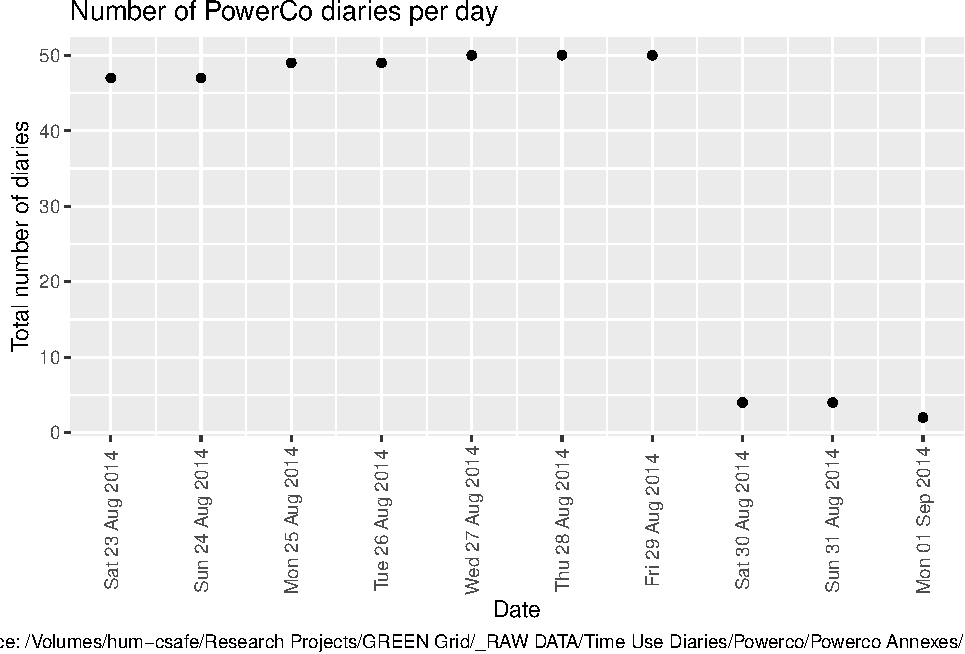
\includegraphics{processNZGGTUDData_files/figure-latex/powerCoDiaryPlot-1.pdf}

\begin{Shaded}
\begin{Highlighting}[]
\NormalTok{ggplot2}\OperatorTok{::}\KeywordTok{ggsave}\NormalTok{(}\KeywordTok{paste0}\NormalTok{(outPath, }\StringTok{"powerCoTUDdates.png"}\NormalTok{))}
\end{Highlighting}
\end{Shaded}

\begin{verbatim}
## Saving 6.5 x 4.5 in image
\end{verbatim}

In total we have 352 diaries from 22 PowerCo households.

\subsection{Unison}\label{unison}

This consists of 5 files found in /Volumes/hum-csafe/Research
Projects/GREEN Grid/\_RAW DATA/Time Use Diaries/Unison/Unison Raw
Data/Raw data with paper diaries included/Cleaned excel data files/:

\begin{itemize}
\tightlist
\item
  TUDAdult\_ONE\_Child\_Unison\_forSAS\_BA.xlsx
\item
  TUDAdult\_TWO\_Children\_Unison\_forSAS\_BA.xlsx
\item
  TUDAdult-THREE-Children-Unison\_forSAS\_BA.xlsx
\item
  TUDAdult-Unison-forSAS\_BA.xlsx
\item
  TUDTeenagerorChild-Unison\_forSAS\_BA.xlsx
\end{itemize}

As before these are copies of the original versions with slight editing
to correct dates and for ease of processing. The relationship between
them is currently unclear!

\begin{Shaded}
\begin{Highlighting}[]
\CommentTok{#fList <- c("TUDAdult_ONE_Child_Unison_forSAS_BA.xlsx", "TUDAdult_TWO_Children_Unison_forSAS_BA.xlsx",}
\CommentTok{#           "TUDAdult-THREE-Children-Unison_forSAS_BA.xlsx", "TUDAdult-Unison-forSAS_BA.xlsx", "TUDTeenagerorChild-Unison_forSAS_BA.xlsx")}

\CommentTok{# load and add sourceFile for easy tracking of errors}
\NormalTok{tudUnison1chDT <-}\StringTok{ }\NormalTok{data.table}\OperatorTok{::}\KeywordTok{as.data.table}\NormalTok{(}\KeywordTok{read_xlsx}\NormalTok{(}\KeywordTok{paste0}\NormalTok{(unisonPath, }\StringTok{"TUDAdult_ONE_Child_Unison_forSAS_BA.xlsx"}\NormalTok{)))}
\NormalTok{tudUnison1chDT}\OperatorTok{$}\NormalTok{sourceFile <-}\StringTok{ "TUDAdult_ONE_Child_Unison_forSAS_BA.xlsx"}
\NormalTok{tudUnison2chDT <-}\StringTok{ }\NormalTok{data.table}\OperatorTok{::}\KeywordTok{as.data.table}\NormalTok{(}\KeywordTok{read_xlsx}\NormalTok{(}\KeywordTok{paste0}\NormalTok{(unisonPath, }\StringTok{"TUDAdult_TWO_Children_Unison_forSAS_BA.xlsx"}\NormalTok{)))}
\NormalTok{tudUnison2chDT}\OperatorTok{$}\NormalTok{sourceFile <-}\StringTok{ "TUDAdult_TWO_Children_Unison_forSAS_BA.xlsx"}
\NormalTok{tudUnison3chDT <-}\StringTok{ }\NormalTok{data.table}\OperatorTok{::}\KeywordTok{as.data.table}\NormalTok{(}\KeywordTok{read_xlsx}\NormalTok{(}\KeywordTok{paste0}\NormalTok{(unisonPath, }\StringTok{"TUDAdult-THREE-Children-Unison_forSAS_BA.xlsx"}\NormalTok{)))}
\NormalTok{tudUnison3chDT}\OperatorTok{$}\NormalTok{sourceFile <-}\StringTok{ "TUDAdult-THREE-Children-Unison_forSAS_BA.xlsx"}
\NormalTok{tudUnisonAdultDT <-}\StringTok{ }\NormalTok{data.table}\OperatorTok{::}\KeywordTok{as.data.table}\NormalTok{(}\KeywordTok{read_xlsx}\NormalTok{(}\KeywordTok{paste0}\NormalTok{(unisonPath, }\StringTok{"TUDAdult-Unison-forSAS_BA.xlsx"}\NormalTok{)))}
\NormalTok{tudUnisonAdultDT}\OperatorTok{$}\NormalTok{sourceFile <-}\StringTok{ "TUDAdult-Unison-forSAS_BA.xlsx"}
\NormalTok{tudUnisonTeenChDT <-}\StringTok{ }\NormalTok{data.table}\OperatorTok{::}\KeywordTok{as.data.table}\NormalTok{(}\KeywordTok{read_xlsx}\NormalTok{(}\KeywordTok{paste0}\NormalTok{(unisonPath, }\StringTok{"TUDTeenagerorChild-Unison_forSAS_BA.xlsx"}\NormalTok{)))}
\NormalTok{tudUnisonTeenChDT}\OperatorTok{$}\NormalTok{sourceFile <-}\StringTok{ "TUDTeenagerorChild-Unison_forSAS_BA.xlsx"}

\NormalTok{nRows <-}\StringTok{ }\KeywordTok{nrow}\NormalTok{(tudUnison1chDT) }\OperatorTok{+}\StringTok{ }\KeywordTok{nrow}\NormalTok{(tudUnison2chDT) }\OperatorTok{+}\StringTok{ }\KeywordTok{nrow}\NormalTok{(tudUnison3chDT) }\OperatorTok{+}\StringTok{ }\KeywordTok{nrow}\NormalTok{(tudUnisonAdultDT) }\OperatorTok{+}\StringTok{ }\KeywordTok{nrow}\NormalTok{(tudUnisonTeenChDT)}
\KeywordTok{print}\NormalTok{(}\KeywordTok{paste0}\NormalTok{(}\StringTok{"Found "}\NormalTok{, }\KeywordTok{tidyNum}\NormalTok{(nRows), }\StringTok{" rows in total"}\NormalTok{))}
\end{Highlighting}
\end{Shaded}

\begin{verbatim}
## [1] "Found 352 rows in total"
\end{verbatim}

Now process the Unison data.

\begin{Shaded}
\begin{Highlighting}[]
\NormalTok{processUnison <-}\StringTok{ }\ControlFlowTok{function}\NormalTok{(dt)\{}
  \CommentTok{# Fix names of variables ----}
  \CommentTok{# do not rename as it's then hard to trace errors}
\NormalTok{  dt <-}\StringTok{ }\NormalTok{dt[, r_diaryDate }\OperatorTok{:}\ErrorTok{=}\StringTok{ `}\DataTypeTok{Choose the date of your diary / entry:}\StringTok{`}\NormalTok{]}
\NormalTok{  dt <-}\StringTok{ }\NormalTok{dt[, code }\OperatorTok{:}\ErrorTok{=}\StringTok{ `}\DataTypeTok{Please enter your designated / CODE}\StringTok{`}\NormalTok{]}

  \CommentTok{# Fix dates ----}
  \CommentTok{#dt <- dt[, r_diaryDate := lubridate::dmy(diaryDate)] # not needed as read_xls gets it right :-)}
  \CommentTok{#dt <- dt[, r_surveyStart := lubridate::dmy_hms(StartDate)]}
  \CommentTok{#dt <- dt[, r_surveyEnd := lubridate::dmy_hms(EndDate)]}
  
  \CommentTok{# Fix hhID ----}
\NormalTok{  dt <-}\StringTok{ }\NormalTok{dt[, tudCode }\OperatorTok{:}\ErrorTok{=}\StringTok{ }\KeywordTok{substr}\NormalTok{(code, }\DecValTok{0}\NormalTok{, }\DecValTok{2}\NormalTok{)] }\CommentTok{# extracts char 1}
\NormalTok{\}}

\NormalTok{tudUnison1chDT <-}\StringTok{ }\KeywordTok{processUnison}\NormalTok{(tudUnison1chDT)}
\NormalTok{tudUnison2chDT <-}\StringTok{ }\KeywordTok{processUnison}\NormalTok{(tudUnison2chDT)}
\NormalTok{tudUnison3chDT <-}\StringTok{ }\KeywordTok{processUnison}\NormalTok{(tudUnison3chDT)}
\NormalTok{tudUnisonAdultDT <-}\StringTok{ }\KeywordTok{processUnison}\NormalTok{(tudUnisonAdultDT)}
\NormalTok{tudUnisonTeenChDT <-}\StringTok{ }\KeywordTok{processUnison}\NormalTok{(tudUnisonTeenChDT)}


\CommentTok{# join them together ----}
\CommentTok{# column name explosion}
\NormalTok{l <-}\StringTok{ }\KeywordTok{list}\NormalTok{(tudUnison1chDT,tudUnison2chDT,tudUnison3chDT,tudUnisonAdultDT,tudUnisonTeenChDT)}
\NormalTok{tudUnisonAllDT <-}\StringTok{ }\NormalTok{data.table}\OperatorTok{::}\KeywordTok{rbindlist}\NormalTok{(l, }\DataTypeTok{fill =} \OtherTok{TRUE}\NormalTok{)}

\CommentTok{# Check for non-parsed diary dates}
\NormalTok{t <-}\StringTok{ }\KeywordTok{head}\NormalTok{(tudUnisonAllDT[}\KeywordTok{is.na}\NormalTok{(r_diaryDate),.(r_diaryDate, tudCode)])}
\NormalTok{knitr}\OperatorTok{::}\KeywordTok{kable}\NormalTok{(}\DataTypeTok{caption =} \StringTok{"Test diaryDates that did not parse"}\NormalTok{, t)}
\end{Highlighting}
\end{Shaded}

\begin{longtable}[]{@{}ll@{}}
\caption{Test diaryDates that did not parse}\tabularnewline
\toprule
r\_diaryDate & tudCode\tabularnewline
\midrule
\endfirsthead
\toprule
r\_diaryDate & tudCode\tabularnewline
\midrule
\endhead
NA & NA\tabularnewline
NA & NA\tabularnewline
NA & NA\tabularnewline
\bottomrule
\end{longtable}

\begin{Shaded}
\begin{Highlighting}[]
\CommentTok{# report edited diary dates (done in .xlsx)}
\NormalTok{t <-}\StringTok{ }\NormalTok{tudUnisonAllDT[}\OperatorTok{!}\KeywordTok{is.na}\NormalTok{(dateNote),.(r_diaryDate, tudCode, dateNote, sourceFile)]}
\NormalTok{knitr}\OperatorTok{::}\KeywordTok{kable}\NormalTok{(}\DataTypeTok{caption =} \StringTok{"Report diaries with edited diary dates (done in .xlsx before loading)"}\NormalTok{, t)}
\end{Highlighting}
\end{Shaded}

\begin{longtable}[]{@{}llll@{}}
\caption{Report diaries with edited diary dates (done in .xlsx before
loading)}\tabularnewline
\toprule
r\_diaryDate & tudCode & dateNote & sourceFile\tabularnewline
\midrule
\endfirsthead
\toprule
r\_diaryDate & tudCode & dateNote & sourceFile\tabularnewline
\midrule
\endhead
2015-07-20 & 28 & imputed &
TUDAdult\_ONE\_Child\_Unison\_forSAS\_BA.xlsx\tabularnewline
2015-07-21 & 28 & imputed &
TUDAdult\_ONE\_Child\_Unison\_forSAS\_BA.xlsx\tabularnewline
2015-07-20 & 33 & imputed &
TUDAdult\_ONE\_Child\_Unison\_forSAS\_BA.xlsx\tabularnewline
2015-07-20 & 39 & imputed &
TUDAdult\_ONE\_Child\_Unison\_forSAS\_BA.xlsx\tabularnewline
2015-07-23 & 39 & imputed &
TUDAdult\_ONE\_Child\_Unison\_forSAS\_BA.xlsx\tabularnewline
2015-07-24 & 39 & imputed &
TUDAdult\_ONE\_Child\_Unison\_forSAS\_BA.xlsx\tabularnewline
2015-07-26 & 39 & imputed &
TUDAdult\_ONE\_Child\_Unison\_forSAS\_BA.xlsx\tabularnewline
2015-07-20 & 39 & imputed &
TUDAdult\_ONE\_Child\_Unison\_forSAS\_BA.xlsx\tabularnewline
2015-07-20 & 41 & might actually be the 20th &
TUDAdult\_TWO\_Children\_Unison\_forSAS\_BA.xlsx\tabularnewline
2015-07-21 & 41 & might actually be the 21st &
TUDAdult\_TWO\_Children\_Unison\_forSAS\_BA.xlsx\tabularnewline
2015-07-20 & 41 & imputed from StartDate &
TUDAdult\_TWO\_Children\_Unison\_forSAS\_BA.xlsx\tabularnewline
2015-07-21 & 41 & imputed from StartDate &
TUDAdult\_TWO\_Children\_Unison\_forSAS\_BA.xlsx\tabularnewline
2015-07-22 & 41 & imputed from StartDate &
TUDAdult\_TWO\_Children\_Unison\_forSAS\_BA.xlsx\tabularnewline
2015-07-23 & 41 & imputed from StartDate &
TUDAdult\_TWO\_Children\_Unison\_forSAS\_BA.xlsx\tabularnewline
2015-07-24 & 41 & imputed from StartDate &
TUDAdult\_TWO\_Children\_Unison\_forSAS\_BA.xlsx\tabularnewline
2015-07-25 & 41 & imputed from StartDate &
TUDAdult\_TWO\_Children\_Unison\_forSAS\_BA.xlsx\tabularnewline
2015-07-26 & 41 & imputed from StartDate &
TUDAdult\_TWO\_Children\_Unison\_forSAS\_BA.xlsx\tabularnewline
2015-07-21 & 31 & corrected to July from Feb &
TUDTeenagerorChild-Unison\_forSAS\_BA.xlsx\tabularnewline
2015-07-26 & 45 & 25/7/2015 missing in original &
TUDTeenagerorChild-Unison\_forSAS\_BA.xlsx\tabularnewline
\bottomrule
\end{longtable}

\begin{Shaded}
\begin{Highlighting}[]
\CommentTok{# Summary table ----}
\NormalTok{t <-}\StringTok{ }\NormalTok{tudUnisonAllDT[, .(}\DataTypeTok{nDiaries =}\NormalTok{ .N,}
                      \DataTypeTok{minDiaryDate =} \KeywordTok{min}\NormalTok{(r_diaryDate),}
                      \DataTypeTok{maxDiaryDate =} \KeywordTok{max}\NormalTok{(r_diaryDate)), keyby =}\StringTok{ }\NormalTok{.(tudCode)]}

\NormalTok{knitr}\OperatorTok{::}\KeywordTok{kable}\NormalTok{(}\DataTypeTok{caption =} \StringTok{"Summary of Unison diaries by household"}\NormalTok{, t)}
\end{Highlighting}
\end{Shaded}

\begin{longtable}[]{@{}lrll@{}}
\caption{Summary of Unison diaries by household}\tabularnewline
\toprule
tudCode & nDiaries & minDiaryDate & maxDiaryDate\tabularnewline
\midrule
\endfirsthead
\toprule
tudCode & nDiaries & minDiaryDate & maxDiaryDate\tabularnewline
\midrule
\endhead
NA & 3 & NA & NA\tabularnewline
28 & 21 & 2015-07-20 & 2015-07-26\tabularnewline
29 & 14 & 2015-07-20 & 2015-07-26\tabularnewline
30 & 14 & 2015-07-20 & 2015-07-26\tabularnewline
31 & 21 & 2015-07-20 & 2015-07-26\tabularnewline
32 & 21 & 2015-07-20 & 2015-07-26\tabularnewline
33 & 14 & 2015-07-20 & 2015-07-26\tabularnewline
34 & 14 & 2015-07-20 & 2015-07-26\tabularnewline
35 & 14 & 2015-07-20 & 2015-07-26\tabularnewline
36 & 14 & 2015-07-20 & 2015-07-26\tabularnewline
37 & 14 & 2015-07-20 & 2015-07-26\tabularnewline
38 & 21 & 2015-07-20 & 2015-07-26\tabularnewline
39 & 21 & 2015-07-20 & 2015-07-26\tabularnewline
40 & 14 & 2015-07-20 & 2015-07-26\tabularnewline
41 & 21 & 2015-07-20 & 2015-07-26\tabularnewline
42 & 21 & 2015-07-20 & 2015-07-26\tabularnewline
43 & 14 & 2015-08-03 & 2015-08-09\tabularnewline
44 & 14 & 2015-07-20 & 2015-07-26\tabularnewline
45 & 37 & 2015-07-20 & 2015-07-26\tabularnewline
46 & 11 & 2015-07-20 & 2015-07-26\tabularnewline
47 & 14 & 2015-07-20 & 2015-07-26\tabularnewline
\bottomrule
\end{longtable}

All of the diaries should be in July/August 2015\ldots{}

\begin{Shaded}
\begin{Highlighting}[]
\NormalTok{myCaption <-}\StringTok{ }\KeywordTok{paste0}\NormalTok{(}\StringTok{"Data source: "}\NormalTok{, unisonPath)}

\NormalTok{plotDT <-}\StringTok{ }\NormalTok{tudUnisonAllDT[, .(}\DataTypeTok{nDiaries =}\NormalTok{ .N), keyby =}\StringTok{ }\NormalTok{.(r_diaryDate)]}
\NormalTok{ggplot2}\OperatorTok{::}\KeywordTok{ggplot}\NormalTok{(plotDT, }\KeywordTok{aes}\NormalTok{(}\DataTypeTok{x =} \KeywordTok{as.Date}\NormalTok{(r_diaryDate), }\DataTypeTok{y =}\NormalTok{ nDiaries)) }\OperatorTok{+}
\StringTok{  }\KeywordTok{geom_point}\NormalTok{() }\OperatorTok{+}
\StringTok{    }\KeywordTok{scale_x_date}\NormalTok{(}\DataTypeTok{date_labels =} \StringTok{"%a %d %b %Y"}\NormalTok{, }\DataTypeTok{date_breaks =} \StringTok{"1 day"}\NormalTok{) }\OperatorTok{+}
\StringTok{  }\KeywordTok{theme}\NormalTok{(}\DataTypeTok{axis.text.x =} \KeywordTok{element_text}\NormalTok{(}\DataTypeTok{angle =} \DecValTok{90}\NormalTok{, }\DataTypeTok{vjust =} \FloatTok{0.5}\NormalTok{, }\DataTypeTok{hjust =} \FloatTok{0.5}\NormalTok{)) }\OperatorTok{+}\StringTok{ }
\StringTok{  }\KeywordTok{labs}\NormalTok{(}\DataTypeTok{title =} \StringTok{"Number of Unison diaries per day"}\NormalTok{,}
       \DataTypeTok{caption =} \KeywordTok{paste0}\NormalTok{(myCaption),}
       \DataTypeTok{x =} \StringTok{"Date"}\NormalTok{,}
       \DataTypeTok{y =} \StringTok{"Total number of diaries"}
    
\NormalTok{  )}
\end{Highlighting}
\end{Shaded}

\begin{verbatim}
## Warning: Removed 1 rows containing missing values (geom_point).
\end{verbatim}

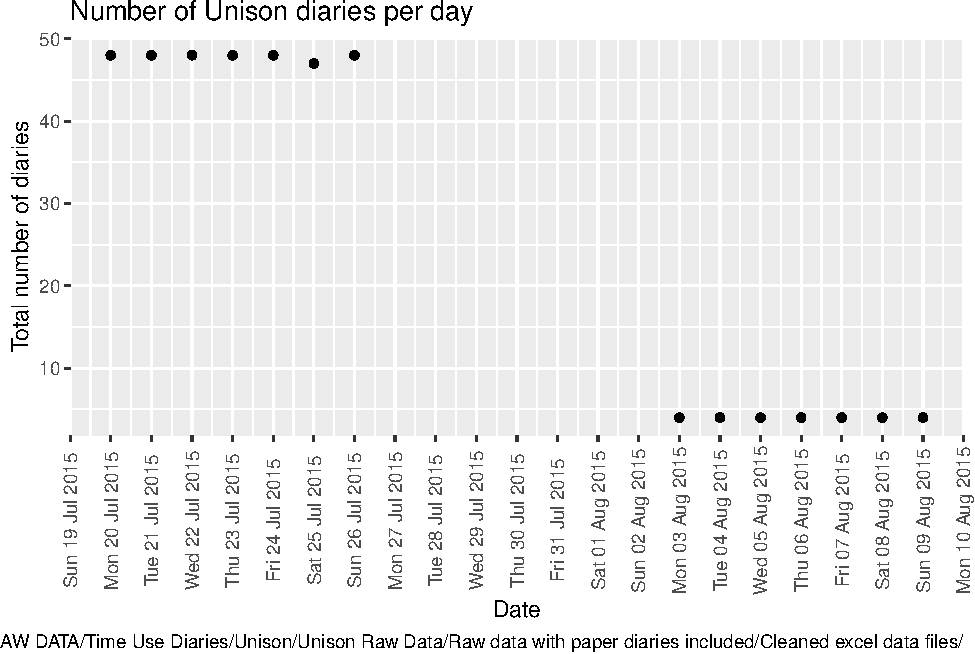
\includegraphics{processNZGGTUDData_files/figure-latex/unisonDiaryPLot-1.pdf}

\begin{Shaded}
\begin{Highlighting}[]
\NormalTok{ggplot2}\OperatorTok{::}\KeywordTok{ggsave}\NormalTok{(}\KeywordTok{paste0}\NormalTok{(outPath, }\StringTok{"unisonTUDdates.png"}\NormalTok{))}
\end{Highlighting}
\end{Shaded}

\begin{verbatim}
## Saving 6.5 x 4.5 in image
\end{verbatim}

\begin{verbatim}
## Warning: Removed 1 rows containing missing values (geom_point).
\end{verbatim}

If any of them are earlier than July 2015 they are flagged below for
ease of fixing.

\begin{Shaded}
\begin{Highlighting}[]
\NormalTok{t <-}\StringTok{ }\NormalTok{tudUnisonAllDT[r_diaryDate }\OperatorTok{<}\StringTok{ "2015-07-01"}\NormalTok{, .(}\DataTypeTok{nDiaries =}\NormalTok{ .N), keyby =}\StringTok{ }\NormalTok{.(r_diaryDate, tudCode, sourceFile)]}
\NormalTok{cap <-}\StringTok{ }\KeywordTok{paste0}\NormalTok{(}\StringTok{"Households with potential diary date errors"}\NormalTok{)}
\NormalTok{knitr}\OperatorTok{::}\KeywordTok{kable}\NormalTok{(}\DataTypeTok{caption =}\NormalTok{ cap, t)}
\end{Highlighting}
\end{Shaded}

Table: Households with potential diary date errors

r\_diaryDate tudCode sourceFile nDiaries ------------ --------
----------- ---------

The tudCodes are \emph{not} the gridSpy ids, we need to create these
from the unison sheet in /Volumes/hum-csafe/Research Projects/GREEN
Grid/\_RAW DATA/TUD\_2\_GridSpyLookup.xlsx.

\begin{Shaded}
\begin{Highlighting}[]
\NormalTok{unisonLinkLUTDT <-}\StringTok{ }\NormalTok{data.table}\OperatorTok{::}\KeywordTok{as.data.table}\NormalTok{(}\KeywordTok{read_xlsx}\NormalTok{(}\KeywordTok{paste0}\NormalTok{(linkLUT), }\DataTypeTok{sheet =} \StringTok{"unison"}\NormalTok{))}

\NormalTok{knitr}\OperatorTok{::}\KeywordTok{kable}\NormalTok{(}\DataTypeTok{caption =} \StringTok{"Linking table"}\NormalTok{, unisonLinkLUTDT)}
\end{Highlighting}
\end{Shaded}

\begin{longtable}[]{@{}rll@{}}
\caption{Linking table}\tabularnewline
\toprule
CODE & tag\_gridSpy\_Hhid & source\tabularnewline
\midrule
\endfirsthead
\toprule
CODE & tag\_gridSpy\_Hhid & source\tabularnewline
\midrule
\endhead
28 & rf\_33 & unison\tabularnewline
29 & rf\_46 & unison\tabularnewline
30 & rf\_37 & unison\tabularnewline
31 & rf\_28 & unison\tabularnewline
32 & rf\_39 & unison\tabularnewline
33 & rf\_29 & unison\tabularnewline
34 & rf\_30 & unison\tabularnewline
35 & rf\_31 & unison\tabularnewline
36 & rf\_43 & unison\tabularnewline
37 & rf\_35 & unison\tabularnewline
38 & rf\_44 & unison\tabularnewline
39 & rf\_41 & unison\tabularnewline
40 & rf\_36 & unison\tabularnewline
41 & rf\_42 & unison\tabularnewline
42 & rf\_34 & unison\tabularnewline
43 & rf\_38 & unison\tabularnewline
43 & rf\_38 & unison\tabularnewline
44 & rf\_32 & unison\tabularnewline
45 & rf\_47 & unison\tabularnewline
46 & rf\_45 & unison\tabularnewline
47 & rf\_40 & unison\tabularnewline
\bottomrule
\end{longtable}

\begin{Shaded}
\begin{Highlighting}[]
\NormalTok{tudUnisonAllDT <-}\StringTok{ }\NormalTok{tudUnisonAllDT[, linkCode }\OperatorTok{:}\ErrorTok{=}\StringTok{ }\KeywordTok{as.character}\NormalTok{(tudCode)]}
\KeywordTok{setkey}\NormalTok{(tudUnisonAllDT, linkCode)}
\NormalTok{unisonLinkLUTDT <-}\StringTok{ }\NormalTok{unisonLinkLUTDT[, linkCode }\OperatorTok{:}\ErrorTok{=}\StringTok{ }\KeywordTok{as.character}\NormalTok{(CODE)]}
\KeywordTok{setkey}\NormalTok{(unisonLinkLUTDT, linkCode)}

\NormalTok{tudUnisonAllDT <-}\StringTok{ }\NormalTok{tudUnisonAllDT[unisonLinkLUTDT] }\CommentTok{# link them}

\NormalTok{tudUnisonAllDT <-}\StringTok{ }\NormalTok{tudUnisonAllDT[, hhID }\OperatorTok{:}\ErrorTok{=}\StringTok{ }\NormalTok{tag_gridSpy_Hhid]}

\CommentTok{# check}

\NormalTok{t <-}\StringTok{ }\NormalTok{tudUnisonAllDT[, .(}\DataTypeTok{nDiaries =}\NormalTok{ .N), keyby =}\StringTok{ }\NormalTok{.(linkCode, hhID)]}
\NormalTok{knitr}\OperatorTok{::}\KeywordTok{kable}\NormalTok{(}\DataTypeTok{caption =} \StringTok{"Check linkage: there should be 1 or 2 diaries for each combination"}\NormalTok{, t)}
\end{Highlighting}
\end{Shaded}

\begin{longtable}[]{@{}llr@{}}
\caption{Check linkage: there should be 1 or 2 diaries for each
combination}\tabularnewline
\toprule
linkCode & hhID & nDiaries\tabularnewline
\midrule
\endfirsthead
\toprule
linkCode & hhID & nDiaries\tabularnewline
\midrule
\endhead
28 & rf\_33 & 21\tabularnewline
29 & rf\_46 & 14\tabularnewline
30 & rf\_37 & 14\tabularnewline
31 & rf\_28 & 21\tabularnewline
32 & rf\_39 & 21\tabularnewline
33 & rf\_29 & 14\tabularnewline
34 & rf\_30 & 14\tabularnewline
35 & rf\_31 & 14\tabularnewline
36 & rf\_43 & 14\tabularnewline
37 & rf\_35 & 14\tabularnewline
38 & rf\_44 & 21\tabularnewline
39 & rf\_41 & 21\tabularnewline
40 & rf\_36 & 14\tabularnewline
41 & rf\_42 & 21\tabularnewline
42 & rf\_34 & 21\tabularnewline
43 & rf\_38 & 28\tabularnewline
44 & rf\_32 & 14\tabularnewline
45 & rf\_47 & 37\tabularnewline
46 & rf\_45 & 11\tabularnewline
47 & rf\_40 & 14\tabularnewline
\bottomrule
\end{longtable}

In total we have 363 diaries from 20 Unison households.

\begin{Shaded}
\begin{Highlighting}[]
\CommentTok{# save out safe file ----}
\NormalTok{ofile <-}\StringTok{ }\KeywordTok{paste0}\NormalTok{(outPath, }\StringTok{"unisonTUDsafe.csv"}\NormalTok{)}
\KeywordTok{print}\NormalTok{(}\KeywordTok{paste0}\NormalTok{(}\StringTok{"Saving Unison cleaned time use diary to "}\NormalTok{, ofile))}
\end{Highlighting}
\end{Shaded}

\begin{verbatim}
## [1] "Saving Unison cleaned time use diary to /Volumes/hum-csafe/Research Projects/GREEN Grid/Clean_data/safe/TUD/unisonTUDsafe.csv"
\end{verbatim}

\begin{Shaded}
\begin{Highlighting}[]
\KeywordTok{write.csv}\NormalTok{(tudUnisonAllDT, ofile)}
\KeywordTok{print}\NormalTok{(}\StringTok{"Done"}\NormalTok{)}
\end{Highlighting}
\end{Shaded}

\begin{verbatim}
## [1] "Done"
\end{verbatim}

\section{Runtime}\label{runtime}

\begin{Shaded}
\begin{Highlighting}[]
\NormalTok{t <-}\StringTok{ }\KeywordTok{proc.time}\NormalTok{() }\OperatorTok{-}\StringTok{ }\NormalTok{startTime}

\NormalTok{elapsed <-}\StringTok{ }\NormalTok{t[[}\DecValTok{3}\NormalTok{]]}
\end{Highlighting}
\end{Shaded}

Analysis completed in 10.474 seconds ( 0.17 minutes) using
\href{https://cran.r-project.org/package=knitr}{knitr} in
\href{http://www.rstudio.com}{RStudio} with R version 3.4.4 (2018-03-15)
running on x86\_64-apple-darwin15.6.0.

\section{R environment}\label{r-environment}

R packages used: data.table, lubridate, ggplot2, readr, dplyr, readxl,
knitr

\begin{itemize}
\tightlist
\item
  base R - for the basics (R Core Team 2016)
\item
  data.table - for fast (big) data handling (Dowle et al. 2015)
\item
  lubridate - date manipulation (Grolemund and Wickham 2011)
\item
  ggplot2 - for slick graphics (Wickham 2009)
\item
  readr - for csv reading/writing (Wickham, Hester, and Francois 2016)
\item
  dplyr - for select and contains (Wickham and Francois 2016)
\item
  knitr - to create this document (Xie 2016)
\item
  greenGridr - for local NZ GREEN Grid utilities
\end{itemize}

\begin{Shaded}
\begin{Highlighting}[]
\KeywordTok{sessionInfo}\NormalTok{()}
\end{Highlighting}
\end{Shaded}

\begin{verbatim}
## R version 3.4.4 (2018-03-15)
## Platform: x86_64-apple-darwin15.6.0 (64-bit)
## Running under: macOS High Sierra 10.13.4
## 
## Matrix products: default
## BLAS: /Library/Frameworks/R.framework/Versions/3.4/Resources/lib/libRblas.0.dylib
## LAPACK: /Library/Frameworks/R.framework/Versions/3.4/Resources/lib/libRlapack.dylib
## 
## locale:
## [1] en_GB.UTF-8/en_GB.UTF-8/en_GB.UTF-8/C/en_GB.UTF-8/en_GB.UTF-8
## 
## attached base packages:
## [1] stats     graphics  grDevices utils     datasets  methods   base     
## 
## other attached packages:
## [1] knitr_1.20          readxl_1.1.0        dplyr_0.7.4        
## [4] readr_1.1.1         ggplot2_2.2.1       lubridate_1.7.4    
## [7] data.table_1.10.4-3 greenGridr_0.1.0   
## 
## loaded via a namespace (and not attached):
##  [1] Rcpp_0.12.16      bindr_0.1.1       magrittr_1.5     
##  [4] hms_0.4.2         munsell_0.4.3     colorspace_1.3-2 
##  [7] R6_2.2.2          rlang_0.2.0.9001  highr_0.6        
## [10] stringr_1.3.0     plyr_1.8.4        tools_3.4.4      
## [13] grid_3.4.4        gtable_0.2.0      htmltools_0.3.6  
## [16] assertthat_0.2.0  yaml_2.1.18       lazyeval_0.2.1   
## [19] rprojroot_1.3-2   digest_0.6.15     tibble_1.4.2     
## [22] bindrcpp_0.2.2    glue_1.2.0        evaluate_0.10.1  
## [25] rmarkdown_1.9     labeling_0.3      stringi_1.1.7    
## [28] cellranger_1.1.0  compiler_3.4.4    pillar_1.2.2     
## [31] scales_0.5.0.9000 backports_1.1.2   pkgconfig_2.0.1
\end{verbatim}

\hypertarget{refs}{}
\hypertarget{ref-data.table}{}
Dowle, M, A Srinivasan, T Short, S Lianoglou with contributions from R
Saporta, and E Antonyan. 2015. \emph{Data.table: Extension of
Data.frame}. \url{https://CRAN.R-project.org/package=data.table}.

\hypertarget{ref-lubridate}{}
Grolemund, Garrett, and Hadley Wickham. 2011. ``Dates and Times Made
Easy with lubridate.'' \emph{Journal of Statistical Software} 40 (3):
1--25. \url{http://www.jstatsoft.org/v40/i03/}.

\hypertarget{ref-baseR}{}
R Core Team. 2016. \emph{R: A Language and Environment for Statistical
Computing}. Vienna, Austria: R Foundation for Statistical Computing.
\url{https://www.R-project.org/}.

\hypertarget{ref-ggplot2}{}
Wickham, Hadley. 2009. \emph{Ggplot2: Elegant Graphics for Data
Analysis}. Springer-Verlag New York. \url{http://ggplot2.org}.

\hypertarget{ref-dplyr}{}
Wickham, Hadley, and Romain Francois. 2016. \emph{Dplyr: A Grammar of
Data Manipulation}. \url{https://CRAN.R-project.org/package=dplyr}.

\hypertarget{ref-readr}{}
Wickham, Hadley, Jim Hester, and Romain Francois. 2016. \emph{Readr:
Read Tabular Data}. \url{https://CRAN.R-project.org/package=readr}.

\hypertarget{ref-knitr}{}
Xie, Yihui. 2016. \emph{Knitr: A General-Purpose Package for Dynamic
Report Generation in R}. \url{https://CRAN.R-project.org/package=knitr}.


\end{document}
